\documentclass[UTF8,a4paper]{ctexart}
\usepackage[margin=1in]{geometry}
\usepackage{fancyhdr,hyperref,float,graphicx}
\pagestyle{fancy}
\hypersetup{hidelinks}

\lhead{\bfseries \leftmark}
\chead{}
\rhead{SCUT}
\lfoot{\url{https://github.com/285571052}}
\cfoot{qhy}
\rfoot{\thepage}
\setlength{\headheight}{13pt}
\renewcommand{\headrulewidth}{0.4pt}
\renewcommand{\footrulewidth}{0.4pt}

\setlength{\parindent}{0pt}
\newcommand{\spaceline}{\vspace{\baselineskip}}

\author{ qhy }
\date{\today}
\title{高性能计算与云计算}

\begin{document}
  \maketitle
  \tableofcontents
  \newpage

  \section{介绍}

  \textbf{高性能与云计算关注的问题:}\\
  如何使计算机更快更方便地解决更大规模的问题。

  \spaceline
  \textbf{做得更快的方法:}
  \begin{enumerate}
    \item [1.] work harder

    换一台更好的计算机

    \item [2.] work smarter

    修改为更加优化的方法

    \item [3.] getting help

    并行处理
  \end{enumerate}

  单核CPU的提升遇到瓶颈,提高计算机性能需要另寻出路:多核时代,由AMD首先推出。

  \spaceline
  \textbf{多核运算的速度一定比单核的CPU快吗?}\\
  不一定,考虑到散热等问题,多核CPU的主频往往比单核的低,若程序只能发挥出一个内核效用的话,
  自然不如单核CPU快。\\
  想要发挥多核功能,设计的软件首先要做并行运算。\\
  多核的出现,使得高性能计算进入普及时代。

  \spaceline
  \textbf{大规模数据处理当前面临的问题:}
  \begin{enumerate}
    \item [1.] 大规模PC集群可靠性差

    一台PC的MTBF(Mean Time Between Failure) = 3年

    则1000台PC的MTBF = 1天

    商用网络 = 低带宽

    这个要求运行系统具备良好的可扩展性、良好的容错能力

    \item [2.] 并行/分布式程序开发、调试困难

    \begin{enumerate}
      \item 数据划分
      \item 任务调度
      \item 任务之间的通信
      \item 错误的处理、容错
    \end{enumerate}

    这要求编程模型具备一定表达能力、很好的简单易用性
  \end{enumerate}

  大数据时代的高性能计算:云计算:通过互联网将资源按需服务的形式提供给用户。

  \spaceline
  \textbf{课程内容}
  \begin{enumerate}
    \item 高性能计算系统与其结构模型
    \item 并行算法设计
    \item 并行程序的设计原理和方法
    \item 云计算
    \item 高性能计算与云计算的应用及发展趋势
  \end{enumerate}

  \spaceline
  \textbf{高性能计算与云计算的3大基础:}
  \begin{enumerate}
    \item 计算

    数据处理能力

    \item 存储

    \item 通信
  \end{enumerate}

  \spaceline
  \textbf{高性能计算与分布式计算的区别?没仔细记,以下瞎写}\\
  高性能计算是把计算任务分配到各个节点上计算\\
  分布式计算则是把各种资源分布在各个节点上计算

  \spaceline
  \textbf{高性能计算的模型框架???没记录,名字也不确定对不对}

  \section{并行结构}
  并行计算机与传统计算机的区别在于其通信架构。\\
  并行计算机的发展体现在:
  \begin{itemize}
    \item 计算借点性能的提高
    \item 节点之间通信的改进
  \end{itemize}

  \begin{figure}[H]
    \centering
    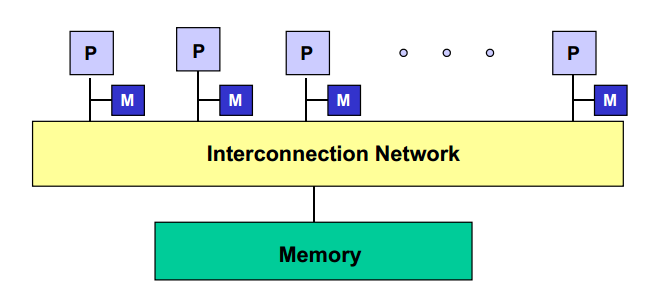
\includegraphics[scale = 0.3]{assets/ParallelComputing_0293e.png}
    \caption{一个通用的并行结构:P表示处理器, M表示本地内存,Memory表示共享内存}
  \end{figure}

  \spaceline
  \textbf{时延:}软件开销 + 通信时延+ 选路时延+ 竞争时延\\
  竞争时延:网络阻塞的时候需要等待。\\
  传输时延:通道时延 + 选路时延

  \spaceline
  \textbf{带宽:}
  \begin{itemize}
    \item 端口带宽\\
    从任意端口到另外端口单位时间内传送消息的最大位数
    \item 聚集带宽\\
    从一半节点到另一半节点,单位时间内传输消息的最大位数
    \item 链路带宽\\
    单位时间内链路传输消息的最大位数
    \item 对剖带宽\\
    每秒钟内,在最小的对剖平面上通过所有连线的最大信息位数。\\
    对剖带宽 = 对剖宽度\footnote{对剖宽度:将网络分成两个相等部分所必须移去的最少边数。对剖宽度越大越好,这样当某个节点故障的时候,整个网络瘫痪的几率就越小} $\times$ 链路带宽
  \end{itemize}

  \spaceline
  \textbf{互联网络的评价标准:}
  \begin{itemize}
    \item 硬件复杂度(Cost)\\
    将N个处理机按一定拓扑结构连成网络所需要的开关的个数
    \item 时延(Latency)\\
    发送消息到接受消息所需的时间
    \item 可扩展性
    \item 容错能力
  \end{itemize}


  \subsection{静态互连网络与动态互连网络}
  \textbf{静态互连网络:}处理单元之间的连接是固定的。
  \begin{itemize}
    \item 一维线性阵列
    \begin{figure}[H]
      \centering
      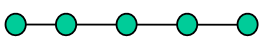
\includegraphics[scale = 0.3]{assets/ParallelComputing_c8f8c.png}
      \caption{一维线性阵列:线,直径:$N-1$,对剖宽度:$1$}
    \end{figure}
    \begin{figure}[H]
      \centering
      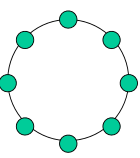
\includegraphics[scale = 0.3]{assets/ParallelComputing_b1923.png}
      \caption{一维线性阵列:环,直径:$\frac{N}{2}$,对剖宽度:$\lfloor 2 \rfloor$}
    \end{figure}
    \item 二维网孔
    \begin{figure}[H]
      \centering
      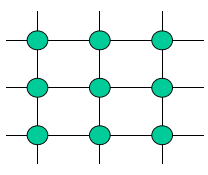
\includegraphics[scale = 0.3]{assets/ParallelComputing_ea5ca.png}
      \caption{二维网孔:网络规模:$N$ , 直径:$2(N^{\frac{1}{2}} - 1)$ , 对剖宽度:$N^{\frac{1}{2}}$}
    \end{figure}
    \begin{figure}[H]
      \centering
      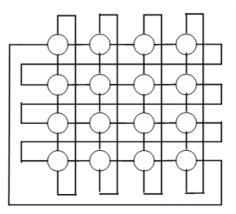
\includegraphics[scale = 0.3]{assets/ParallelComputing_5b5f4.png}
      \caption{Illiac 网孔:垂直方向上带环绕,水平方向呈蛇形状,
      网络规模:$N$ , 直径:$N^{\frac{1}{2}} - 1$ , 对剖宽度:$2N^{\frac{1}{2}}$}
    \end{figure}
    \begin{figure}[H]
      \centering
      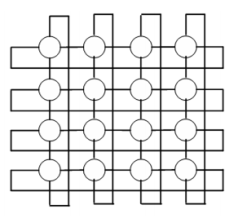
\includegraphics[scale = 0.3]{assets/ParallelComputing_d6701.png}
      \caption{2D环绕:垂直方向和水平方向都带环绕。
      网络规模:$N$ , 直径:$2\lfloor \frac{N^{\frac{1}{2}}}{2} \rfloor$ , 对剖宽度:$2N^{\frac{1}{2}}$}
    \end{figure}
    \item 树\\
    \textbf{星型网络:}是树的一个特殊情况。\\
    \textbf{胖树:}传统多叉树,根节点容易成为通信的瓶颈,因为带宽不够,胖树则是越靠近根带宽越大。
    \begin{figure}[H]
      \centering
      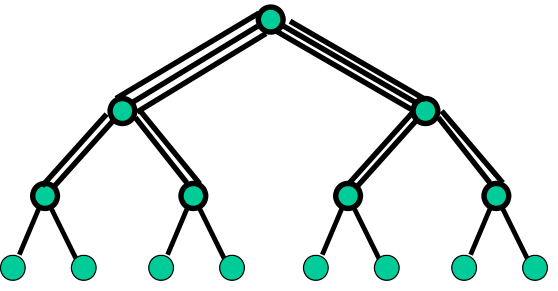
\includegraphics[scale = 0.3]{assets/ParallelComputing_3e1c8.png}
      \caption{Fat-Trees}
    \end{figure}
    \item 超立方\\
    一个n-立方由$N = 2^n$个顶点组成。直径为$n$,对剖宽度为$\frac{N}{2}$
    \begin{figure}[H]
      \centering
      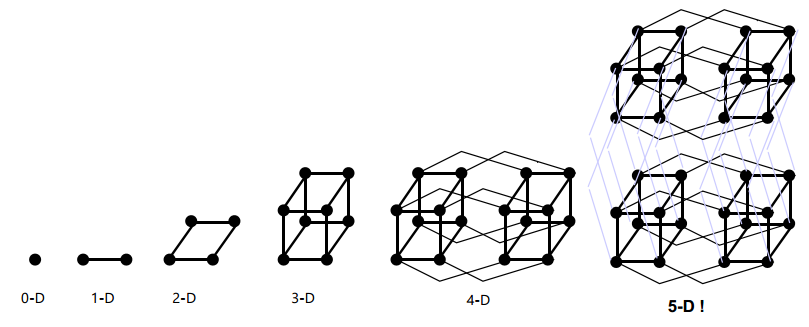
\includegraphics[scale = 0.3]{assets/ParallelComputing_9924c.png}
      \caption{超立方}
    \end{figure}
    \item 立方环\\
    将超立方上的节点使用一个环代替。
    \begin{figure}[H]
      \centering
      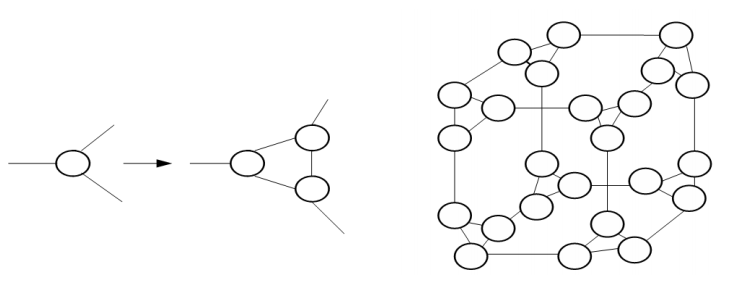
\includegraphics[scale = 0.3]{assets/ParallelComputing_b9cb4.png}
      \caption{3-立方环}
    \end{figure}
    \item 蝶形网络
    \begin{figure}[H]
      \centering
      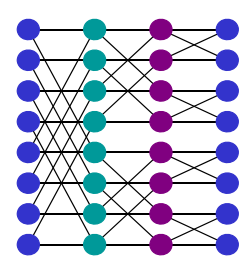
\includegraphics[scale = 0.4]{assets/ParallelComputing_00400.png}
      \caption{蝶网:规模:$N = (k+1)2^k$ , 直径:$2k$ , 对剖宽度:$2^k$}
    \end{figure}

  \end{itemize}

  \begin{figure}[H]
    \centering
    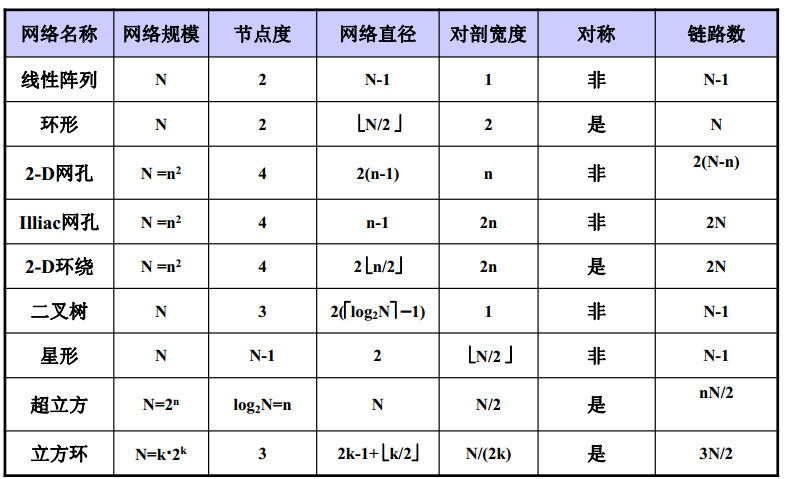
\includegraphics[scale = 0.5]{assets/ParallelComputing_3087c.png}
    \caption{静态互联网络特性比较}
  \end{figure}

  \textbf{小结:}
  \begin{itemize}
    \item 节点度越大,连接性越好,但网络越复杂,成本越高
    \item 一般静态网络节点度小于4
    \item 对剖宽度越大越好
    \item 网络尽可能对称,这样便于管理
    \item 对称性影响可扩展性与路由效率
  \end{itemize}

  \spaceline
  \textbf{动态互连网络:}连接可以动态地变换,用交换开关构建。
  \begin{itemize}
    \item 总线\\
    成本低,不随处理器数目的增加而增加\\
    扩展性不好,总线的带宽固定,随着处理器数增多,每个处理器带宽减少\\
    可利用程序中的局部性原理减少对总线带宽的需求
    \item 多叉开关\\
    任意两点之间有一个开关,对应两个状态on和off\\
    具备良好的宽带特性,带宽独享,完全非阻塞通讯\\
    但是代价大$O(n^2)$\\
    有两种使用方式,一:处理器间通信,二:处理器和存储模块之间的存取\\
    \item 多级互连网络\\
    多个交叉开关级联起来\\
    \textbf{交换开关模块}:允许一对多的连接,但不允许多对一的连接(即单一方向)
  \end{itemize}

  \begin{figure}[H]
    \centering
    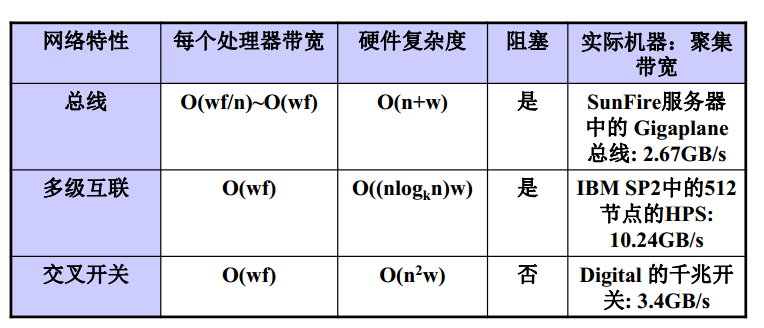
\includegraphics[scale = 0.5]{assets/ParallelComputing_3cbfc.png}
    \caption{动态互联网络比较,n:节点规模,w:数据宽度,f:时钟频率}
  \end{figure}

  \spaceline
  \textbf{标准互联网络}
  \begin{itemize}
    \item 以太网
    \item InfiniBand
  \end{itemize}

\end{document}
